\section{Results}\label{sec:results}

\subsection{Held-out likelihood}
Table~\ref{tab:fits} reports the log-likelihoods on the training and held-out days.
Static context improves the held-out log-likelihood by \GainStatic\ per event over the timetable alone, mostly through the strong preference for classmates.
Network context adds \GainNetwork\ per event (M2 over M1).
Memory adds \GainMemoryAlone\ per event without network context (M6 over M1) and \GainMemoryWithNetwork\ per event with it (M5 over M2), so that network context absorbs only \MemoryAbsorbed\% of the memory effect, while it still adds \GainNetworkWithMemory\ per event when memory is present (M5 over M6).
With two time scales of memory, the Markovian model M3 falls short of the aging model C1 by \ConeOverMthree\ log-likelihood units on the held-out days; with four time scales, M5 exceeds C1 by \MfiveOverCone\ units.
A Markovian description with network context and traces on several time scales therefore predicts held-out contacts at least as well as intrinsic power-law aging.

\begin{table*}[t]
\caption{Log-likelihoods $L$ on the training days (Monday to Wednesday) and the held-out days (Thursday and Friday), held-out improvement per event relative to M1, and the Kolmogorov--Smirnov distance (KS) of the time-rescaled contact durations on the held-out days from the unit exponential distribution (zero for a correct model).}
\label{tab:fits}
\begin{ruledtabular}
\begin{tabular}{llrrrrr}
model & components & param. & $L$ (training) & $L$ (held out) & $\Delta L$/event & KS \\
\colrule
M0 & timetable & 22 & $-$368\,997 & $-$235\,337 & $-0.987$ & 0.186 \\
M1 & M0 + static context & 28 & $-$302\,346 & $-$194\,943 & $+0.000$ & 0.180 \\
M2 & M1 + network & 32 & $-$288\,045 & $-$186\,055 & $+0.217$ & 0.163 \\
M4 & M1 + memory (2) & 34 & $-$253\,614 & $-$161\,772 & $+0.810$ & 0.112 \\
M3 & M2 + memory (2) & 38 & $-$243\,554 & $-$155\,741 & $+0.957$ & 0.111 \\
M6 & M1 + memory (4) & 38 & $-$247\,207 & $-$157\,675 & $+0.910$ & 0.102 \\
M5 & M2 + memory (4) & 42 & $-$237\,010 & $-$151\,601 & $+1.058$ & 0.090 \\
C1 & M1 + power-law aging & 33 & $-$240\,850 & $-$152\,158 & $+1.045$ & 0.119 \\
\end{tabular}
\end{ruledtabular}

\end{table*}

\subsection{Estimated effects}
Table~\ref{tab:estimates} shows the estimates of the best model M5 (probability units; a coefficient $b$ multiplies the rate by about $e^{4b}$ per unit of its count).
Classmates form contacts about \ClassFactor\ times as often as other pairs, and each common current contact multiplies the formation rate by about \TriFactor, so that contacts form predominantly within existing groups.
Common contacts lower the termination rate (groups stabilize contacts), whereas more current contacts of either student raise both rates.
The memory terms combine to a termination hazard that is raised during the first few minutes of a contact and lowered afterwards, and to a re-formation rate that is suppressed during the first half minute after a contact ended (which the definition of contacts by gaps of at least 40 seconds excludes) and strongly raised during the following minutes.
In C1, the corresponding power-law exponents are \ConeTermExponent\ for termination and \ConeFormExponent\ for re-formation.

\begin{table}[t]
\caption{Estimates (probability units) and standard errors (observed information) of the network-context and memory effects of model M5 on the formation and termination rates of contacts.
The timetable effects are not shown.}
\label{tab:estimates}
\begin{ruledtabular}
\begin{tabular}{lrrrr}
 & \multicolumn{2}{c}{formation} & \multicolumn{2}{c}{termination} \\
effect & estimate & s.e. & estimate & s.e. \\
\colrule
same class & $0.882$ & $0.006$ & $-0.001$ & $0.006$ \\
Facebook friends & $0.062$ & $0.004$ & $-0.013$ & $0.004$ \\
survey friendship & $0.070$ & $0.003$ & $-0.017$ & $0.002$ \\
common contact & $0.762$ & $0.009$ & $-0.186$ & $0.005$ \\
other current contact & $0.112$ & $0.002$ & $0.036$ & $0.002$ \\
met on earlier day & $0.148$ & $0.004$ & $-0.008$ & $0.003$ \\
memory, $\delta = 2$/min & $-2.790$ & $0.034$ & $-0.504$ & $0.010$ \\
memory, $\delta = 0.5$/min & $1.529$ & $0.019$ & $0.699$ & $0.010$ \\
memory, $\delta = 0.1$/min & $0.042$ & $0.007$ & $-0.129$ & $0.004$ \\
memory, $\delta = 0.02$/min & $0.087$ & $0.001$ & $0.002$ & $0.001$ \\
\end{tabular}
\end{ruledtabular}

\end{table}

\subsection{Time-rescaling residuals}
No model passes the time-rescaling test, but the residuals improve in the same order as the held-out likelihood (Table~\ref{tab:fits}, Fig.~\ref{fig:residuals}): the KS distance falls from \KSMone\ for M1 to \KSMfive\ for M5, while C1 reaches \KSCone.
The rescaled durations are too rare near zero and too frequent between about 0.1 and 0.4: the models overestimate the hazard at the very start of a contact and underestimate it at intermediate ages.

\begin{figure}[t]
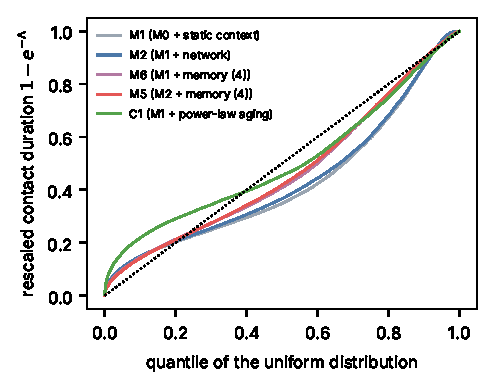
\includegraphics[width=\columnwidth]{generated/fig-residuals}
\caption{Time-rescaling diagnostic on the held-out days: quantiles of $1 - e^{-\Lambda}$, with $\Lambda$ the integrated termination hazard of each contact under the fitted model, against the quantiles of the uniform distribution.
A correct model lies on the diagonal.}
\label{fig:residuals}
\end{figure}

\subsection{Sensitivity to the definition of contacts}\label{sec:sensitivity}
Merging records with gaps of up to 120 seconds instead of 40 seconds into one contact reduces the number of contacts by a third and changes the size, but not the order, of the effects (Table~\ref{tab:sensitivity}).
Memory still dominates, but its gain without network context falls from \GainMemoryAloneTwo\ to \GainMemoryAloneLong\ per event (two time scales, M4 over M1), so that a part of the short-term memory reflects contacts that are interrupted by detection failures rather than ended.
Network context gains \GainNetworkLong\ per event with the longer gaps.
The advantage of the aging model shrinks more: with the longer gaps, C1 gains \ConeLong\ per event over M1 and falls behind the Markovian model M3 with two memory time scales (\MthreeLong\ per event), so that a part of the apparent power-law aging also reflects interrupted contacts.

\begin{table}[t]
\caption{Sensitivity to the definition of contacts: held-out log-likelihood and improvement per event relative to M1 with gaps of up to 120 seconds merged into one contact, and the improvement per event with gaps of up to 40 seconds (Table~\ref{tab:fits}) for comparison.}
\label{tab:sensitivity}
\begin{ruledtabular}
\begin{tabular}{lrrr}
model & $L$ (held out) & $\Delta L$/event & $\Delta L$/event, 40-s gaps \\
\colrule
M0 & $-$175\,221 & $-0.955$ & $-0.987$ \\
M1 & $-$148\,269 & $+0.000$ & $+0.000$ \\
M2 & $-$140\,726 & $+0.267$ & $+0.217$ \\
M4 & $-$130\,737 & $+0.621$ & $+0.810$ \\
M3 & $-$124\,936 & $+0.827$ & $+0.957$ \\
C1 & $-$128\,071 & $+0.715$ & $+1.045$ \\
\end{tabular}
\end{ruledtabular}

\end{table}
